\subsection{函数图形的描绘}
\paragraph{}
借助于一阶导数的符号,可以确定函数图形在哪个区间上上升,哪个区间上下降,在什么地方有极值点。
\paragraph{}
借助于二阶导数的符号,可以确定函数图形在哪个区间上为凹,在哪个区间上为凸,在什么地方有拐点。知道函数图形的升降、凹凸以及极值点和拐点后,也就可以掌握函数的性态。

\paragraph{}
\begin{enumerate}
  \item 确定定义域,及函数具有的特性(奇偶性、周期性等),并求出一阶导数$f'(x)$和二阶导数$f''(x)$;
  \item 求出一阶导数和二阶导数在定义域的全部零点,并求出函数$f(x)$的间断点及$f'(x)$和$f''(x)$不存在的点,划分函数的定义域;
  \item 确定这些部分区间内$f'(x)$和$f''(x)$的符号,并由此确定函数图形的升降和凹凸,极值点和拐点;
  \item 算出$f'(x)$和$f''(x)$的零点以及不存在的点所对应的函数值,定出图形上相应的点;为了把图形描绘得准确些,有时还需要补充一些点;然后结合第$3$、$4$步中得到的结果,联结这些点画出函数$y=f(x)$的图形。
\end{enumerate}

\subsection{例子}
\paragraph{}
\textbf{例子1\;}画出函数$y=x^3-x^2-x+1$的图形

\paragraph{}
\textbf{解}

\bgroup
\def\arraystretch{1.5}
\setlength\tabcolsep{0.3cm}
\begin{figure}[H]
\centering
  \begin{tabular}{c|c|c|c|c|c|c|c}
    \hline
    $x$ & $(-\infty,-\frac{1}{3})$ & $-\frac{1}{3}$ & $(-\frac{1}{3},\frac{1}{3})$ & $\frac{1}{3}$
    & $(\frac{1}{3},1)$ & $1$ & $(1,+\infty)$ \\
    \hline
    $f'(x)$ & $+$ & $0$ & $-$ & $-$ & $-$ & $0$ &$+$ \\
    \hline
    $f''(x)$ & $-$ & $-$ & $-$ & $0$ & $+$ & $+$ & $+$ \\
    \hline
    $y=f(x)\text{的图形}$ &
    {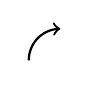
\begin{tikzpicture}[scale=0.4,thick]
      \draw [->,domain=180:90] plot ({cos(\x)}, {sin(\x)});
    \end{tikzpicture}} & 极大 &
    {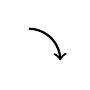
\begin{tikzpicture}[scale=0.4,thick]
      \draw [->,domain=90:0] plot ({cos(\x)}, {sin(\x)});
    \end{tikzpicture}} & 拐点 &
    {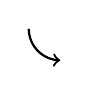
\begin{tikzpicture}[scale=0.4,thick]
      \draw [->,domain=180:270] plot ({cos(\x)}, {sin(\x)});
    \end{tikzpicture}} & 极小 &
    {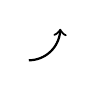
\begin{tikzpicture}[scale=0.4,thick]
      \draw [->,domain=-90:0] plot ({cos(\x)}, {sin(\x)});
    \end{tikzpicture}} \\
    \hline
  \end{tabular}
\end{figure}
\egroup
